\documentclass[addpoints]{exam}

\usepackage{verbatim, multicol, tabularx,hyperref, tikz}
\usepackage{amsmath,amsthm, amssymb, stmaryrd, latexsym, bm, listings, qtree}

\lstset{
  extendedchars=\true,
  inputencoding=utf8,
  literate=
  {é}{{\'{e}}}1
  {è}{{\`{e}}}1
  {ê}{{\^{e}}}1
  {ë}{{\¨{e}}}1
  {û}{{\^{u}}}1
  {ù}{{\`{u}}}1
  {â}{{\^{a}}}1
  {à}{{\`{a}}}1
  {î}{{\^{i}}}1
  {ô}{{\^{o}}}1
  {ç}{{\c{c}}}1
  {Ç}{{\c{C}}}1
  {É}{{\'{E}}}1
  {Ê}{{\^{E}}}1
  {À}{{\`{A}}}1
  {Â}{{\^{A}}}1
  {Î}{{\^{I}}}1
  {Ö}{{\"O}}1
  {Ä}{{\"A}}1
  {Ü}{{\"U}}1
  {ö}{{\"o}}1
  {ä}{{\"a}}1
  {ü}{{\"u}}1
  {ß}{{\ss}}1
  ,
  aboveskip=1mm,
  belowskip=1mm,
  showstringspaces=false,
  columns=flexible,
  basicstyle={\scriptsize\ttfamily},
  numbers=left,
  frame=single,
  framextopmargin=0pt,
  framexbottommargin=0pt,
  breaklines=true,
  breakatwhitespace=true,
  keywordstyle=\color{blue},
  identifierstyle=\color{violet},
  stringstyle=\color{teal},
  commentstyle=\color{darkgray}
}

\hypersetup{colorlinks=true,urlcolor=blue}

\headheight = 0.05 in
\headsep = 0.05 in
\parskip = 0.05in
\parindent = 0.0in
\floatsep = 0.05in

\DeclareMathOperator*{\argmin}{arg\!min}
\DeclareMathOperator*{\argmax}{arg\!max}

\title{Midterm Review}
\author{CS 4277: Deep Learning}
\date{}

\begin{document}
\maketitle

\begin{questions}

\question According to Tom Mitchell, machine learning is the study of algorithms that

\begin{itemize}
\item improve their performance {\tt P}
\item at some task {\tt T}
\item with experience {\tt E}.
\end{itemize}

A well-defined learning task is given by {\tt <P, T, E>}.

Formulate the following problems according to Tom Mitchell's machine learning problem specification (see \href{https://drcs.codes/deep-learning/slides/machine-learning.pdf}{Machine Learning Slides}) and the specification our textbook. For each of the following problems specify:

\begin{itemize}
\item The task {\tt T},
\item The performance measure {\tt P},
\item The experience {\tt E},
\item The target function $f: \mathcal{X} \rightarrow \mathcal{Y}$, that is,
\begin{itemize}
\item the input space $\mathcal{X}$, and
\item the output space $\mathcal{Y}$.
\end{itemize}
\end{itemize}

Remember that a function maps a domain to a co-domain, and these domains are sets.

\question Medical diagnosis: A patient walks in with a medical history and some symptoms, and you want to identify the problem.

\ifprintanswers
\begin{solution}
\begin{itemize}
\item Task, {\tt T}: diagnose problem
\item Performance, {\tt P}: diagnosis is correct or incorrect
\item Experience, {\tt E}: $<medical-history, symptoms>$
\item Target function $f: \mathcal{X} \rightarrow \mathcal{Y}$:
\begin{itemize}
\item $\mathcal{X} = \{\vec{x} \vert x_1 \in \{family-history-heart-disease\}, x_2 \in \mathbb{R} = cholesterol-level \}$ and other such features
\item $\mathcal{Y} = \{disease_1, disease_2, ..., disease_n \}$
\end{itemize}
\end{itemize}
\end{solution}
\else
\vspace{3in}
\fi

\newpage

\question For a single neuron with a two-dimensional input $\bm{x}$ and single scalar output $y$, formulate the preactivation value using a linear algebra operation.  Don't forget to account for the bias.


\ifprintanswers
\begin{solution}

\begin{equation}
  \bm{x}^T\bm{\theta} =
  \left[\begin{array}{ccc}
  1 & x_1 & x_2
  \end{array}\right]
  \left[\begin{array}{c}
  \theta_0 \\ \theta_2 \\ \theta_2
  \end{array}\right]
  =\sum_{i=1}^{D}x_i \theta_i
\end{equation}

\end{solution}
\else
\vspace{2in}
\fi

\question Write a mathematical definition of the ReLU activation function.

\ifprintanswers
\begin{solution}

\begin{equation}
  a(z) = RelU(z) =
  \begin{cases}
  0, & z < 0\\
  z, & z \ge 0
  \end{cases}
\end{equation}

\end{solution}
\else
\vspace{2in}
\fi

\question The squared error loss function for a regression model with a single scalar input and single scalar output is:

\begin{equation}
    L(\bm{\phi}) = \sum_{i=1}^{I} (\phi_0 + \phi_1 x_i - y_i)^2
\end{equation}

Write the squared error loss function for a regression model with a two-dimensional vector input, $\bm{x}$, and a single scalar output $y$.

\ifprintanswers
\begin{solution}
    \begin{equation}
        L(\bm{\phi}) = \sum_{i=1}^{I} (\phi_0 + \phi_1 x_{i1} + \phi_2 x_{i2} - y_i)^2
    \end{equation}
\end{solution}
\else
\vspace{1.5in}
\fi

\newpage

\question Given the following shallow neural network:

\begin{center}
  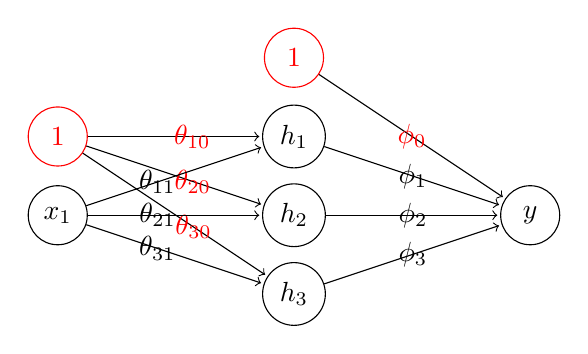
\begin{tikzpicture}[shorten >=1pt,->]
  \tikzstyle{unit}=[draw,shape=circle,minimum size=.75cm]


  % Input layer
  \node[unit,style=red](inone) at (0,2){$1$};
  \node[unit](x) at (0,1){$x_1$};

  % Hidden layer
  \node[unit,style=red](hone) at (3,3){$1$};
  \node[unit](h1) at (3,2){$h_1$};
  \node[unit](h2) at (3,1){$h_2$};
  \node[unit](h3) at (3,0){$h_3$};

  % Output
  \node[unit](y) at (6,1){$y$};

  % Connections
  \draw (inone) to node [style=red, pos=0.6]{$\theta_{10}$} (h1);
  \draw (inone) to node [style=red, pos=0.6]{$\theta_{20}$} (h2);
  \draw (inone) to node [style=red, pos=0.6]{$\theta_{30}$} (h3);
  \draw (x) to node [pos=0.4]{$\theta_{11}$} (h1);
  \draw (x) to node [pos=0.4]{$\theta_{21}$} (h2);
  \draw (x) to node [pos=0.4]{$\theta_{31}$} (h3);

  \draw (hone) to node [style=red]{$\phi_0$} (y);
  \draw (h1) to node {$\phi_1$} (y);
  \draw (h2) to node {$\phi_2$} (y);
  \draw (h3) to node {$\phi_3$} (y);

  \end{tikzpicture}
  \end{center}

  Write a single equation for the network $y = f(x, \vec{\phi}$ with parameters $\bm{\phi} = \{\bm{\theta}, \bm{\phi}\}$.

  \ifprintanswers
  \begin{solution}

    \begin{equation}
      y = f(x, \vec{\phi}) = \phi_0 + \phi_1 a(\theta_{10} + \theta_{11}x) + \phi_2 a(\theta_{20} + \theta_{21}x) + \phi_3 a(\theta_{30} + \theta_{31}x)
    \end{equation}

  \end{solution}
  \else
  \vspace{1.5in}
  \fi

  \question State the universal approximation theorem.

  \ifprintanswers
  \begin{solution}
    For any function, there exits a shallow network with enough hidden units to approximate the function to any precision.
  \end{solution}
  \else
  \vspace{1.5in}
  \fi

  \question A shallow network with $D > 2$ hidden units can create up to how many linear regions?

  \ifprintanswers
  \begin{solution}
    \[
    D+1
    \]
  \end{solution}
  \else
  \vspace{1.5in}
  \fi

  \question A deep network with $K$ layers of $D > 2$ hidden units can create up to how many linear regions?

  \ifprintanswers
  \begin{solution}
    \[
    (D+1)^K
    \]
  \end{solution}
  \else
  \vspace{1.5in}
  \fi

  \question Explain the {\it depth efficiency} of deep networks vs shallow networks.

  \ifprintanswers
  \begin{solution}
    Some functions require exponentially more hidden units in a shallow network than an equivalent deep network.
  \end{solution}
  \else
  \vspace{1.5in}
  \fi

  \question Explain the i.i.d. assumption.

  \ifprintanswers
  \begin{solution}
    We assume training data points are drawn independently and are identically-distributed.
  \end{solution}
  \else
  \vspace{1.5in}
  \fi

  \question What is a loss function?

  \ifprintanswers
  \begin{solution}
    A loss function returns a single number that represents the mismatch between the model's output $\hat{y}$ and the ground truth $y$.
  \end{solution}
  \else
  \vspace{1.5in}
  \fi

  \question How do machine learning algorithms use loss functions?

  \ifprintanswers
  \begin{solution}
    A machine learning algorithm minimizes the loss function, which represents the best possible mapping from training inputs to outputs.
  \end{solution}
  \else
\vspace{1.5in}
  \fi

  \question Write a concise general mathematical formulation of the goal of a machine learning algorithm that relates the model's parameters to the loss function.

  \ifprintanswers
  \begin{solution}
    \[
    \bm{\hat{\phi}} = \argmin_{\bm{\phi}}(L(\bm{\phi}))
    \]
  \end{solution}
  \else
  \vspace{1.5in}
  \fi

  \question Write the general 2-step gradient descent algorithm.

  \ifprintanswers
  \begin{solution}
    1. Compute the derivatives of the loss with respect to the parameters.
    \[
    \nabla L
    =
    \frac{\partial L}{\partial \bm{\phi}}
    =
    \left[
    \begin{array}{c}
      \frac{\partial L}{\partial \bm{\phi}_0}\\
      \frac{\partial L}{\partial \bm{\phi}_1}\\
      \vdots\\
      \frac{\partial L}{\partial \bm{\phi}_N}
    \end{array}
    \right]
    \]
    2. Update the parameters according to the update rule:
    \[
    \bm{\phi}  \leftarrow \bm{\phi} - \alpha \frac{\partial L}{\partial \bm{\phi}}
    \]
    where $\alpha$ is a positive scalar value called the {\it learning rate} that controls how large parameter updates are in each training step.
  \end{solution}
  \else
  \vspace{5in}
  \fi

  \question What are local minima?  What is the global minimum?

  \ifprintanswers
  \begin{solution}
    The global minimum is the point at which the function's value is minimal.  Local minima are points at which the function's value is lower than it's neighbors, but not as low as the global minimum.  In this case gradient descent is guaranteed to converge to the global minimum given suitable learning rate.
  \end{solution}
  \else
  \vspace{1.5in}
  \fi

  \question What if the learning rate is set too high?

  \ifprintanswers
  \begin{solution}
    Won't converge to minimum because updates will "jump over" the minimum.
  \end{solution}
  \else
  \vspace{1.5in}
  \fi

  \question Is full-batch gradient descent guaranteed to find the global minimum?  Why or why not?

  \ifprintanswers
  \begin{solution}
    No.  If the loss function has local minima in addition to the global minimum, full-batch gradient descent may converge to a local minimum.  If there are many local minima or the parameters happen to be initialized nearer to a local minumum than the global minimum, the chances of converging to a local minimum increase.
  \end{solution}
  \else
  \vspace{1.5in}
  \fi

  \question Describe stochastic gradient descent and how it improves on full-batch gradient descent.

  \ifprintanswers
  \begin{solution}
    At each iteration, the algorithm chooses a random subset of the training data and computes the gradient from these examples alone. This subset is known as a minibatch or batch for short.  Batches are drawn without replacement, and iterations continue with new batches until all training data points have been used -- an epoch.

    Beacause the gradient is computed on a subset of the data, the direction of parameter updates might not be the steepest descent, or may actually be a "climb" with respect to the full data set.  This has the effect of "climbing out" of regions of local minima.  SGD is not guaranteed to find the global minimum, but in practice SGD gives good results.
  \end{solution}
  \else
  \vspace{1.5in}
  \fi

  \question Describe SGD modified with momentum and the purpose of momentum.

  \ifprintanswers
  \begin{solution}

  \end{solution}
  \else
  \vspace{1.5in}
  \fi

  \question Describe Adam and its purpose.

  \ifprintanswers
  \begin{solution}

  \end{solution}
  \else
  \vspace{1.5in}
  \fi

  \question What are the components of the Hessian matrix?

  \ifprintanswers
  \begin{solution}
    The second derivatives of the loss function witih respect to the model parameters.
  \end{solution}
  \else
  \vspace{1.5in}
  \fi

  \question What is useful about the Hessian matrix?

  \ifprintanswers
  \begin{solution}
    If the Hessian matrix is positive definite, that is, all its eigenvalues are positive for any parameter values, then the loss function is convex, meaning it has a single global minimum with no local minima.
  \end{solution}
  \else
  \vspace{1.5in}
  \fi

  \question What is computed in the forward pass of the backpropagation algorithm?

  \ifprintanswers
  \begin{solution}
    The input is {\it fed forward} to compute all intermediate values: all the preactivations, $f_k$, and activations, $h_k$, the output, and the loss, $y - \hat{y}$, are computed and stored.
\end{solution}
\else
\vspace{1.5in}
\fi

  \question What is computed in the backward pass of the backpropagation algorithm?

  \ifprintanswers
  \begin{solution}
    The derivatives of the loss $\ell_i$ with respect to the intermediate values computed in the forward pass, then the derivatives of the loss $\ell_i$ with respect to the parameters $\beta_k$ and $\omega_k$.
\end{solution}
\else
\vspace{1.5in}
\fi

\question Describe the efficiency of the backpropagation algorithm with respect to time and memory.

  \ifprintanswers
  \begin{solution}
    Backpropagation is efficient with respect to time but requires a great deal of storage to store intermediate values.
\end{solution}
\else
\vspace{1.5in}
\fi

\question How are the weights of a network initialized?

  \ifprintanswers
  \begin{solution}
    With values drawn from a Guassian with $\mu = 0$ and some $\sigma^2$.
  \end{solution}
\else
\vspace{1.5in}
\fi

\question Describe the vanishing gradients problem and what initialization mistake leads to it.

  \ifprintanswers
  \begin{solution}
  \end{solution}
\else
\vspace{1.5in}
\fi

\question Describe the exploding gradients problem and what initialization mistake leads to it.

  \ifprintanswers
  \begin{solution}
  \end{solution}
\else
\vspace{1.5in}
\fi

\question What initialization method avoids the vanishing gradients and exploding gradients problem?

  \ifprintanswers
  \begin{solution}
  \end{solution}
  \else
  \vspace{1.5in}
  \fi




\end{questions}

\end{document}
